\section{Blog Appendix}

\subsection{Automated Solution to the Blog Challenge}\label{SolutionBlog}

The automated solution script simulates the player’s journey from step 1 until flag retrieval. The key steps include:

\begin{itemize}
    \item Reading starting IATA code.
    \item Downloading an image file from the travel blog.
    \item Extracting GPS coordinates and date stamp from EXIF metadata.
    \item Using this data to deduce the return flight.
    \item Searching after the flight with the flight tracker and identifying the correct flight number.
    \item Assembling and outputting the flag in the format \texttt{flag\{DEPARTUREIATACODE\_FLIGHTNUMBER\}}.
\end{itemize}

The following snippets illustrate this process:

\begin{minted}[linenos]{bash}
STARTINGPOINT=$(curl --insecure "https://web1.$DOMAIN" | grep -o "CPH")
wget --no-check-certificate "https://web1.$DOMAIN/pictures/p12.png" -O "$OUTPUT_FILE"
GPS=$(exiftool "$OUTPUT_FILE" -n | grep "GPS.Position" | sed 's/.*: //')
DATE=$(exiftool "$OUTPUT_FILE" | grep "Date/Time.Original" | awk '{print $4}' | sed 's/:/-/g')
\end{minted}
\begin{listing}[H]
\caption{Metadata extraction from blog image}
\end{listing}

\begin{minted}[linenos]{bash}
if [ "$GPS" == "35.769272 140.389898" ]; then 
	IATA="NRT"
	fi
echo "IATA AIRPORT for the Challenge Picture: $IATA"
\end{minted}
\begin{listing}[H]
\caption{Simulating using Google Maps to insert coordinates, to get the corresponding airport(IATA code)}
\end{listing}


\begin{minted}[linenos]{bash}
SEARCHURL=$"https://web2.$DOMAIN/index.php?departingAirport=$IATA&
    arrivingAirport=$STARTINGPOINT"
RESPONSE=$(curl --insecure -s "$SEARCHURL")
FLIGHTNUMBER=$(echo "$RESPONSE" | grep -oP "[A-Z]{2}[0-9]{3}(?=\\s*<br><strong>Departure:</strong>\\s*NRT\\
    s+at\\s+$DATE)")
\end{minted}
\begin{listing}[H]
\caption{Flight lookup on the simulated tracker}
\end{listing}

\begin{minted}[linenos]{bash}
FLAG="flag{"$IATA"_"$FLIGHTNUMBER"}"
echo "$FLAG" > /run/solution/flag.txt
cat /run/solution/flag.txt
\end{minted}
\begin{listing}[H]
\caption{Flag generation and output}
\end{listing}

\begin{minted}[linenos]{bash}
#!/bin/bash

# Logs the domain being used for the challenge
echo "Trying to echo Domain: $DOMAIN"

# -------------------------------
# Setup: Setting up variables and urls.
# -------------------------------
IMAGE_URL2="https://$DOMAIN/pictures/p12.png"
OUTPUT_FILE="pic.png"                                                                                                   
URL="https://$DOMAIN"


# -------------------------------
# Step 1: Extracting airport code from the blog page.
# -------------------------------
STARTINGPOINT=$(curl --insecure "https://blog.$DOMAIN" | grep -o "CPH")
echo "Starting Point for Prof. PP: $STARTINGPOINT"


# -------------------------------
# Step 2: Download picture containing Metadata
# -------------------------------
# Using wget to getting the accesible picture on website 1  
wget --no-check-certificate "https://blog.$DOMAIN/pictures/p12.png" -O "$OUTPUT_FILE"
echo "Downloaded picture saved as: $OUTPUT_FILE"

\end{minted}
\begin{listing}[H]
\caption{The whole blog solution part 1}
\end{listing}

\begin{minted}[linenos]{bash}
# -------------------------------
# Step 3: Extract Metadata from image, such as GPS and Date.
# -------------------------------
# Extracting information in it's raw form so it can be used again
GPS=$(exiftool "$OUTPUT_FILE" -n | grep "GPS.Position" | sed 's/.*: //')
echo "GPS Locations: $GPS"
DATE=$(exiftool "$OUTPUT_FILE" | grep "Date/Time.Original" | awk '{print $4}' | sed 's/:/-/g')
echo "Time Create: $DATE"
# ---------------------------------------------------
# Step 4: Finding out IATA airport code based on GPS from image
# ---------------------------------------------------
# Simulating going onto google maps, and pasting the GPS Coordinates, where after looking at the map, to realise the closest AIRPORT
if [ "$GPS" == "35.769272 140.389898" ]; then 
	IATA="NRT"
	fi
echo "IATA AIRPORT for the Challenge Picture: $IATA"
# ---------------------------------------------------
# Step 5: Search on the flight log service webpage, for flight info.
# ---------------------------------------------------
SEARCHURL=$"https://flight-logs.$DOMAIN/index.php?departingAirport=$IATA
    &arrivingAirport=$STARTINGPOINT"
echo "Searching flight logs at: $SEARCHURL"
RESPONSE=$(curl --insecure -s "$SEARCHURL")
# ---------------------------------------------------
# Step 6: Extract flight number using regex
# ---------------------------------------------------
FLIGHTNUMBER=$(echo "$RESPONSE" | grep -oP "[A-Z]{2}[0-9]{3}(?=\\s*<br><strong>Departure:</strong>
    \\s*NRT\\s+at\\s+$DATE)")
echo "Print Flight Number: $FLIGHTNUMBER"
# ---------------------------------------------------
# Step 7: Format and save flag
# ---------------------------------------------------
FLAG="flag{"$IATA"_"$FLIGHTNUMBER"}"
echo "$FLAG" > /run/solution/flag.txt
echo "The flag saved in /run/solution/flag.txt is: $(cat /run/solution/flag.txt)"
\end{minted}
\begin{listing}[H]
\caption{The whole blog solution part 2}
\end{listing}

\subsection{Image of Airport (p12.png)}\label{apx:p12}

\begin{figure}[H]
    \centering
    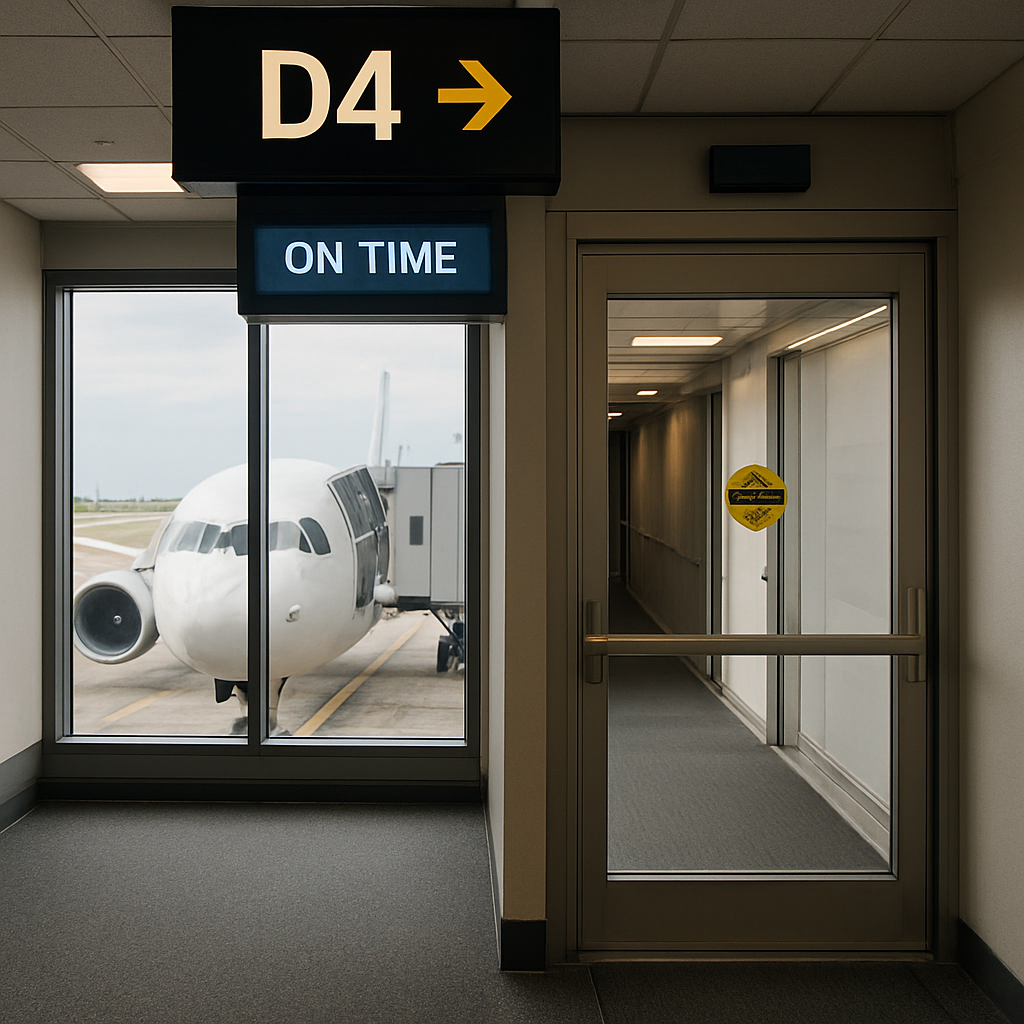
\includegraphics[width=0.75\linewidth]{img/p12.png}
    \caption{AI Generated Airport Picture}
    \label{fig:p12}
\end{figure}
